\documentclass{standalone}

\begin{document}
\chapter*{Introduction}\addcontentsline{toc}{chapter}{Introduction}
\markboth{INTRODUCTION}{}

Colorectal cancer is a malignant neoplasm of the large intestine resulting from the uncontrolled proliferation of the cells making up the colorectal tract.
Colorectal cancer is the second malignant tumor per number of deaths after lung cancer and the third per number of new cases after breast and lung cancer\cite{cancerstats}.
It is estimated that, in EU-27 countries in 2020, colorectal cancer accounted for $12.7 \%$ of all new cancer diagnoses and $12.4\%$ of all deaths due to cancer\cite{eucancerstats}. 
\\

\begin{figure}[!ht]
	\centering
	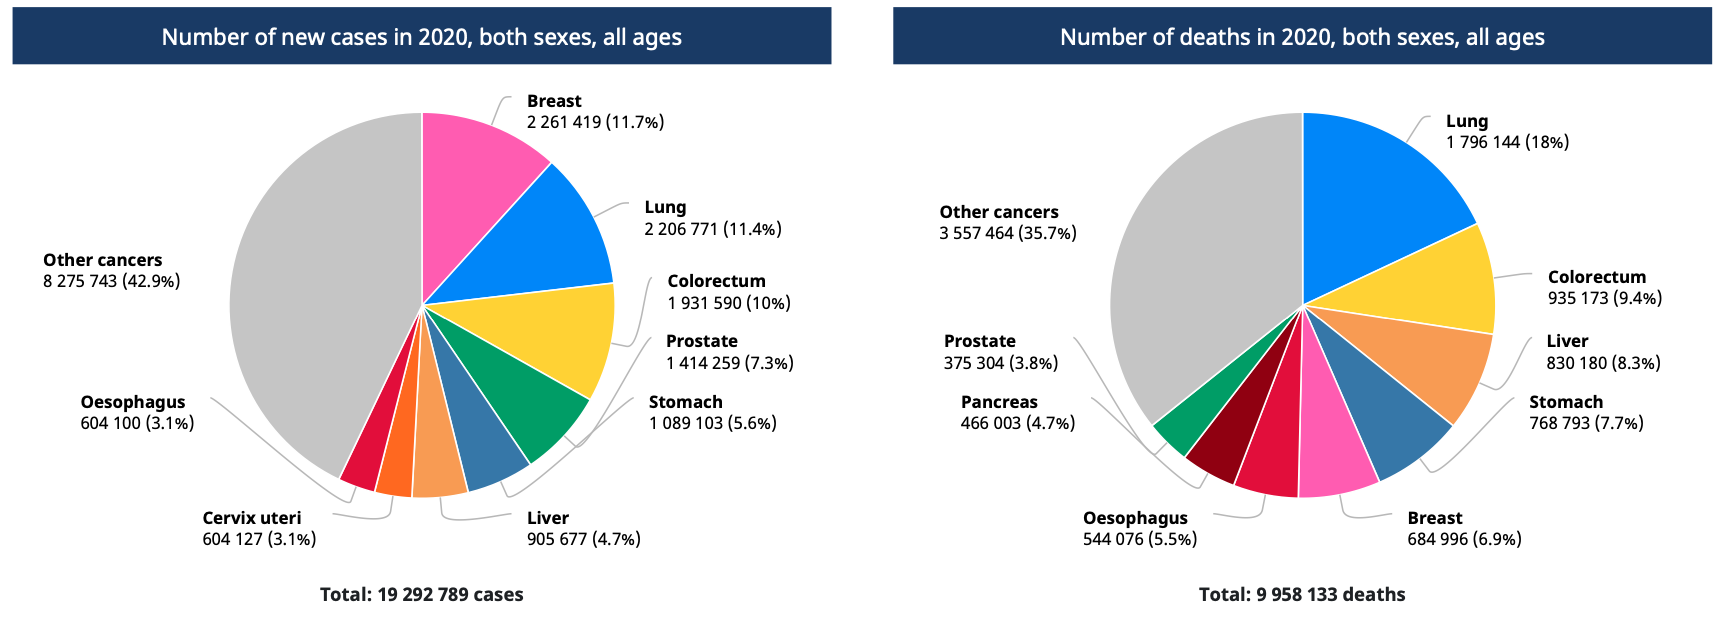
\includegraphics[width=\linewidth]{../images/cancerstats.png}
	\caption{World's cancer cases and deaths in 2020. As you can see from the \textit{Left} image, colorectal cancer is the third malignant tumor per number of new cases after breast and lung cancer while as shown on the \textit{Right} image, it is the second one per number of deaths after lung cancer. From \textit{International Agency for Research on Cancer}\cite{cancerstats}. }
\end{figure}

Among the risk factors for this kind of cancer, non-hereditary ones range from colon polyps to long-standing ulcerative colitis, from Crohn's disease to old age. 
Moreover, genetic history (HNPCC or Lynch syndrome) and nutritional factors as diabetes II can increase the probability of developing colorectal cancer \cite{tesicoppola}.
\\
\begin{figure}[!ht]
	\centering
	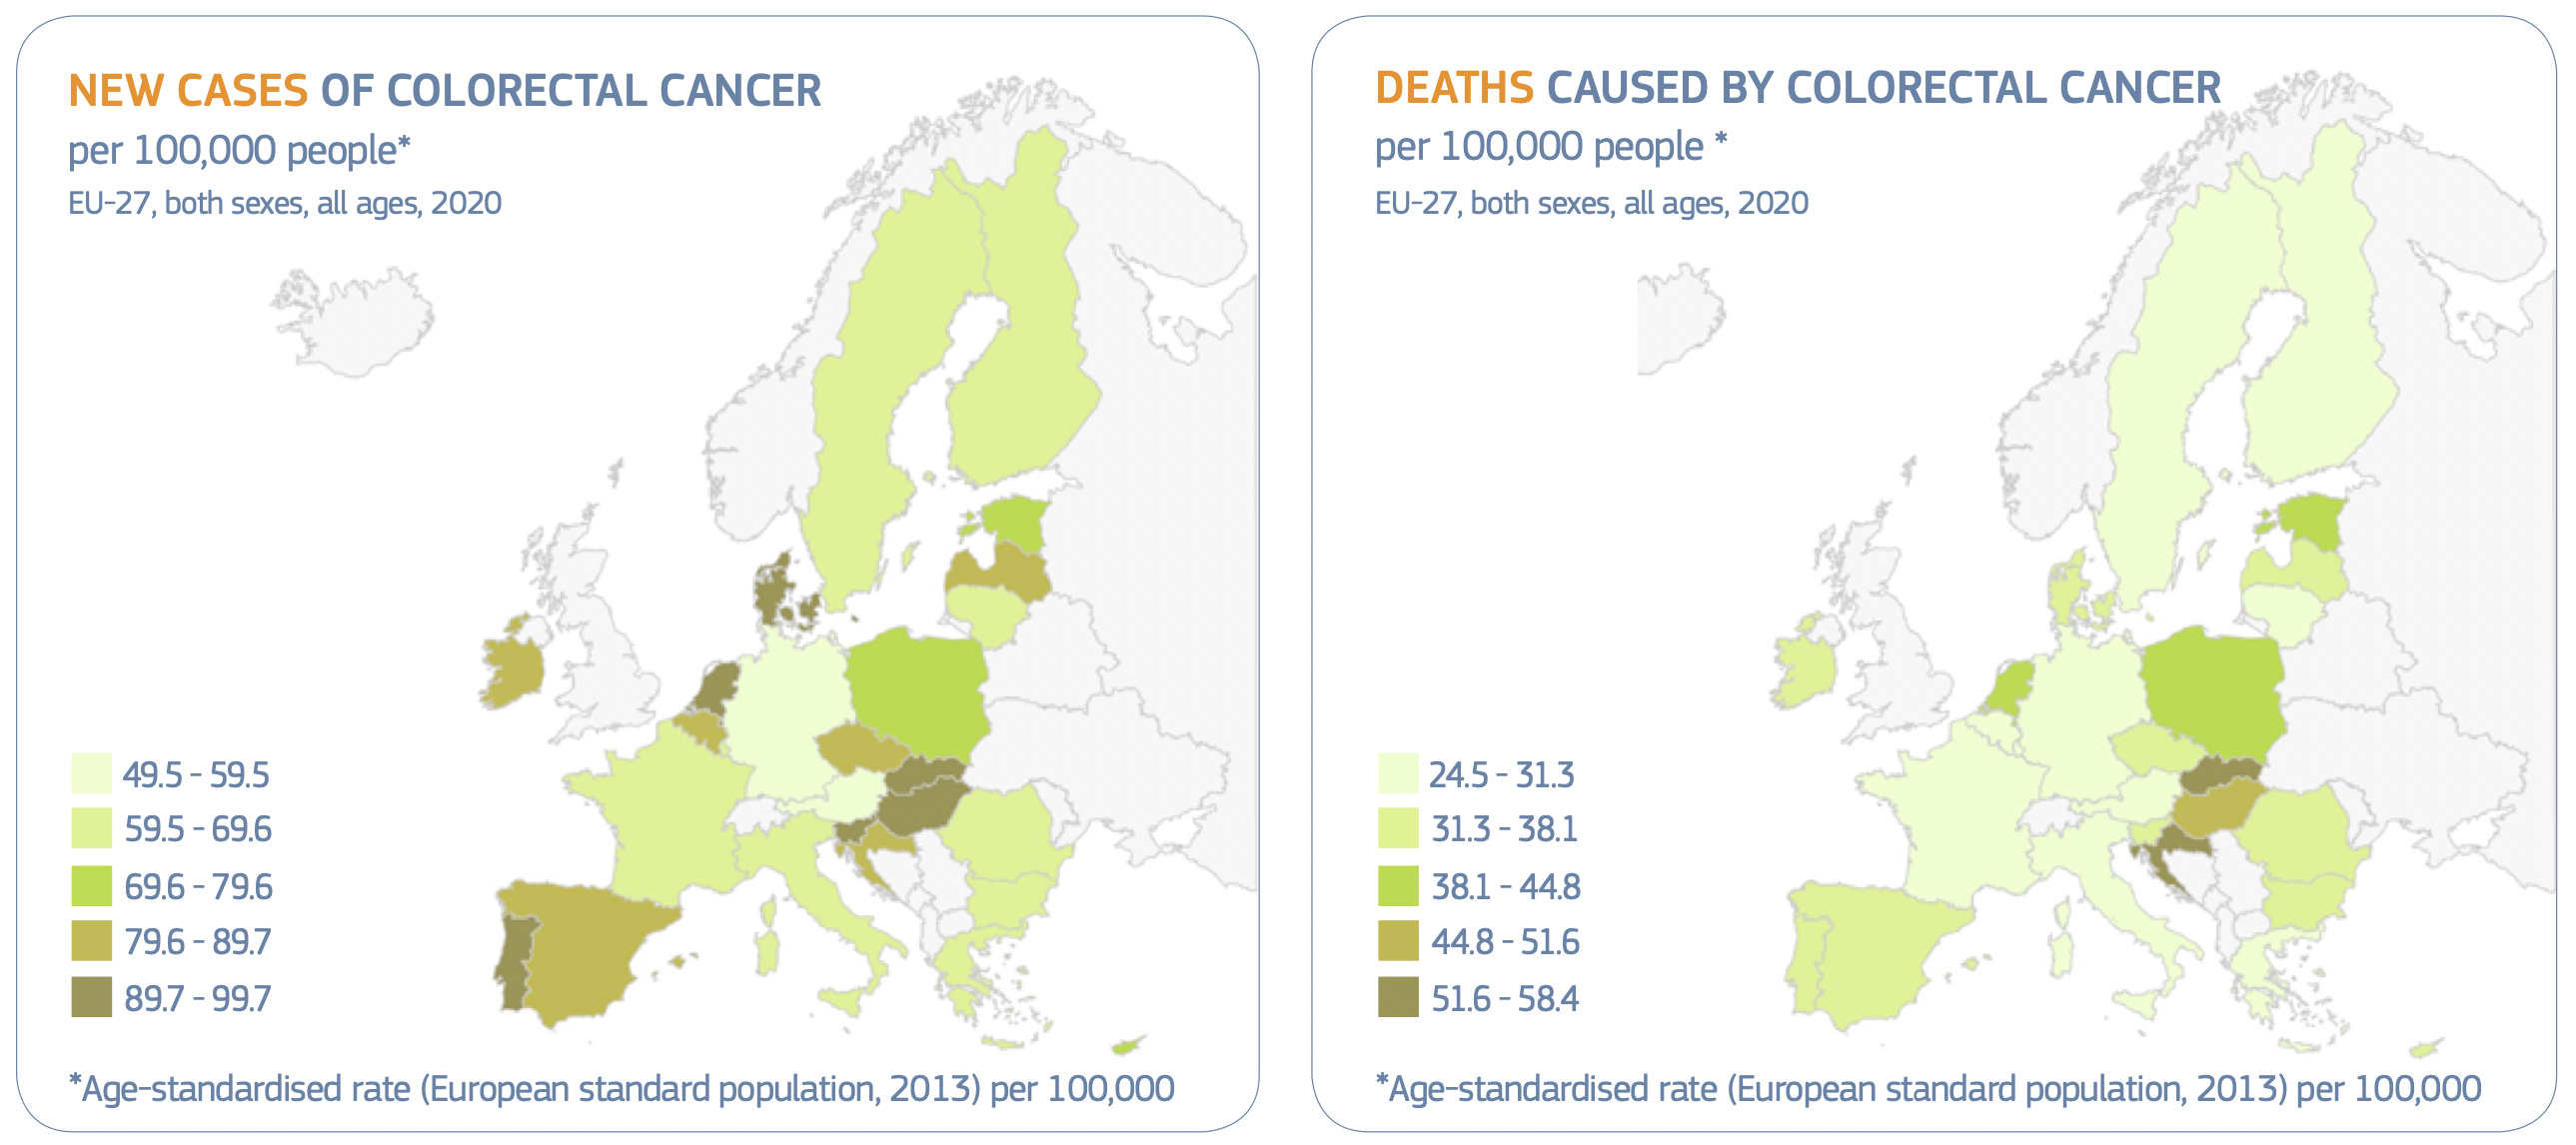
\includegraphics[width=\linewidth]{../images/distribmap.png}
	\caption{ EU-27 countries' distribution map of colorectal cancer cases and deaths in 2020 per $100.000$ people (both sex, all ages). \textit{Left)}: EU-27 countries' new cases of colorectal cancer. \textit{Right)}: EU-27 countries' deaths caused by colorectal cancer. From \textit{ECIS – European Cancer Information System}\cite{eucancerstats}.}
\end{figure}

Preventive measures for colorectal cancer include physical activity, reducing the consumption of processed meat and alcohol, and avoiding smoking\cite{stats2019}.
\\
Screening and diagnosis methods for colorectal cancer involve different techniques. 
The gold standard in medical routines is the colonoscopy which is an invasive technique\cite{jovana}.
Among medical imaging techniques, Magnetic Resonance Imaging (MRI) and Computed Tomography (CT) are the most used\cite{tesicoppola}. 
In particular, Magnetic Resonance Imaging (MRI) is used for pre-operative identification and for the evaluation of the neoadjuvant chemo-radiotherapy of patients affected by colorectal cancer\cite{tesicoppola}.

\begin{figure}[!htp]

    \centering
    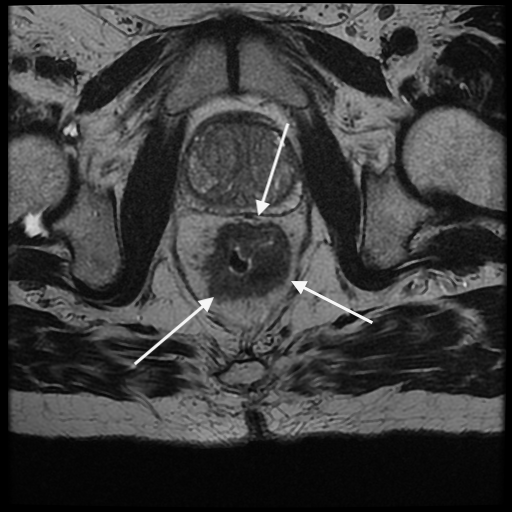
\includegraphics[width=.49\textwidth]{../images/BO11_slice_13.png}\hfill
    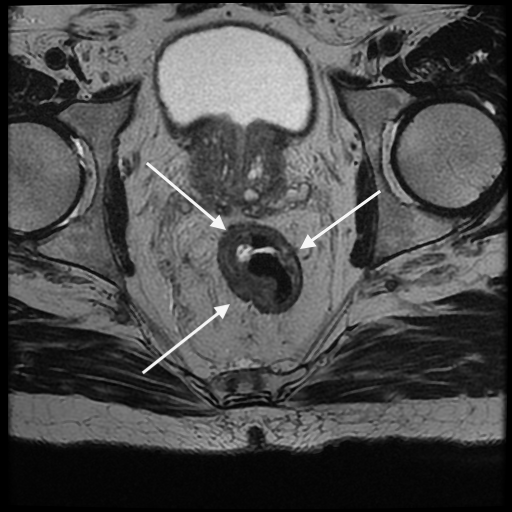
\includegraphics[width=.49\textwidth]{../images/BO11_slice_5.png}\hfill
    
\caption{Axial T2-weighted Magnetic Resonance images of colorectal tract. The images provide a view from the transverse (or axial) plane of the colorectal tract, highlighting fat (low signal) and water (high signal) within the body. The tumor region is denoted by the arrows.
From IRCCS Sant’Orsola-Malpighi Policlinic Dataset.}
\label{trittico}
    
\end{figure}

In order to get information about diagnosis, therapy evaluation, stage of colorectal cancer, analysis on radiological images can be performed through dedicated algorithms.
\\
In this scenario, the correct and fast identification of the cancer regions is a fundamental task.
This can be achieved by using segmentation techniques.
The results of segmentation can be used to perform radiomic features extraction, which can provide fundamental information about organs or lesion volumes, to monitor the evolution of a particular disease, and/or to evaluate the effects of therapeutical treatment.
Therefore, segmentation plays a crucial role for clinicians in identifying diseases such as tumors.
Up to now, this task is performed by using manual or semi-automatic techniques which are time-consuming (requiring hours per day) since it requires interaction with trained specialists.\cite{tesicoppola, jovana}.
Moreover, the obtained results are highly sensitive to the specialist expertise.
Therefore, the reproducibility of the same results is not always possible\cite{Trebeschi2017}.

To overcome these issues, an automated and fast approach is required.
\\
Nowadays, Artificial Intelligence (AI) technologies, such as deep learning models, are exploited with impressive results.
Particularly in the field of biomedical imaging, Convolutional neural networks (CNNs) are one of the deep-learning-based approaches largely exploited for detection and segmentation purposes\cite{Trebeschi2017}.
\\
The state-of-art about Convolutional neural networks for colorectal cancer segmentation purposes on MRI scans is not very wide like other topics about this field.
Anyways, it comes out that colorectal cancer segmentation on MRI scans is very challenging due to many issues such as low-contrast appearance of cancerous regions, the complex peri-tumoral background, class-imbalance\cite{YiJieHuang}.
\\
Different approaches have been proposed in literature.
Trebeschi et al. \cite{Trebeschi2017}, proposed a deep learning approach for fully-automated localization and segmentation of rectal cancer by using \textit{ad hoc} convolutional neural network based on T2-weighted MRI and diffusion-weighted (DWI) scans. 
\\
Despite the good results, this approach requires the implementation of a particular convolutional neural network and DWI scans, which are not always performed in clinical routines.
Moreover, Yi-Jie Huang\cite{YiJieHuang} showed that good results can be obtained also without DWI scans by changing the loss function of the network.
They studied the effect of changing the loss function of the same segmentation model on T2-weighted MRI scans, showing that a proper loss function can improve the segmentation performance.
\\
Another issue to take into account is the presence of \textit{mucinous} cases, that is a tumor subtype characterized by bright tumoral areas on MRI scans, different from the \textit{adenocarcinomas} characterized by dark tumoral areas.
In fact, as showed by Panic et al.\cite{jpanic}, \textit{mucinous} cases can considerably affect the performance of the implemented convolutional neural network.
\\
Another approach, proposed by Xiaoling Pang et al.\cite{XiaolingPang} bases the automatic segmentation in two phases: locating automatically the tumor region on the MRI scans and performing segmentation on the located areas.
\\
In the end, regardless of the approach, such automatic alternatives would also facilitate the extraction of radiomic features, where complex tumor phenotypical characteristics can be quantified and correlated to diagnostic or prognostic factors\cite{Trebeschi2017}.
This was performed both by Bulens et al.\cite{Bulens} and by Xiaoling Pang et al.\cite{XiaolingPang} involving radiomic features with the pathologic complete response (pCR) after neoadjuvant chemo-radiotherapy of patients affected by locally advanced rectal cancer (LARC).
\\
They were not the only ones to involve radiomic features with a possible cancer evaluation.
Somoro et al. \cite{haralick} showed that radiomic features can be exploited on T2-weighted colorectal MRI scans for a possible cancer evaluation. 
In particular how they correlate to Stage Malignancy.
\\
Also a study of Zhihui Li\cite{ZhihuiLi}, showed how MRI-based radiomic-features predictive models were constructed to assess the tumor regression grade (TRG) and pathologic complete response (pCR), respectively.
\\
However in most of the cases, radiomic features are extracted after segmentation performed manually by expert operators or by using semi-manual techniques. 
\\
The aim of this project is to develop and apply an automated pipeline for the segmentation of MRI scans of patients affected by colorectal cancer in order to predict the response to neoadjuvant chemo-radiotherapy by using radiomic features. 
Here, we propose an approach based on segmentation and radiomic features extraction.
The segmentation process exploits a Convolutional Neural Network like U-Net to perform automatic segmentation of the tumor regions.
Then, the results of segmentation are used to perform radiomic features extraction to obtain the prediction of response, based on the Tumor Regression Grade (TRG).
The work was developed and validated on MRI scans provided by IRCCS Sant’Orsola-Malpighi Polyclinic.
\\
This dissertation will start from the materials and methods.
Firstly, we will focus on medical digital images, the general properties of medical digital images, and the DICOM format.
After that, it will be the turn of the performed pre-processing techniques.
They consist of a denoising technique and a gamma correction to remove possible noise sources and improve the image contrast, respectively.
Moreover, we will cover the topic of segmentation, providing to the reader a description of Thresholding, Convolutional Neural Networks and U-Net.
Then, we will talk about radiomics and its possible purposes.
Even an overview of Principal Component Analysis and Support Vector Classifiers will be provided.
To conclude the materials and methods chapter, we will see the main methods used to evaluate the obtained results.
Among them, we find the Dice Similarity Coefficient (DSC), the confusion matrix and the ROC curve.
\\
Dissertation will continue describing the main pipeline characteristics and its structure.
Firstly, we will cover the description of the pipeline workflow.
In particular, about how each step of the pipeline workflow was achieved and performed, from the pre-processing of the images to the prediction of the response to neoadjuvant chemo-radiotherapy.
This chapter will focus both on the pipeline description and implementation. 
\\
The obtained results will be presented in the aimed chapter.
After a description of the dataset provided by the IRCCS Sant’Orsola-Malpighi Polyclinic, the performance of the pipeline will be checked respectively for the segmentation task and for the prediction of response.
Moreover, the possible outputs of the implemented pipeline will be shown.
\\
Finally, the results and some possible developments will be discussed in the conclusions.
\\
A comparison between two different segmentation models will be discussed in the Appendix of this text.


\end{document}